\documentclass[a4paper,12pt]{article}

\usepackage[
    left=2cm,
    right=2cm,
    top=3cm,
    bottom=3cm
]{geometry}

\usepackage[utf8]{inputenc}
\usepackage[czech]{babel}
\usepackage[T1]{fontenc}
\usepackage{graphicx}
\usepackage{array}
\usepackage{booktabs}
\usepackage{tabularx}
\usepackage{makecell}
\usepackage{float}
\usepackage{newunicodechar}
\usepackage{url}
\usepackage{siunitx}
\usepackage{listings}
\usepackage{xcolor}
\usepackage{diagbox}
\usepackage{hyperref}
\usepackage{tikz}
\usepackage{pgfplots}
\usepackage{amsmath}

\pgfplotsset{compat=1.18}

\usepackage{fancyhdr}
\pagestyle{fancy}

\fancyhf{}
\fancyhead[L]{ARI -- Úkol 1}
\fancyhead[R]{Pavel Pernička}
\fancyfoot[C]{\thepage}

\fancypagestyle{firstpage}{
    \fancyhf{}
    \renewcommand{\headrulewidth}{0pt}
    \renewcommand{\footrulewidth}{0pt}
    \fancyfoot[C]{\thepage}
}


\definecolor{myblue}{RGB}{111,0,248}
\newcommand{\colorcircle}[1]{%
  \tikz[baseline=-0.6ex]\draw[fill=#1,draw=none] (0,0) circle (1.5ex);%
}
\newcommand{\unitC}{\,^\circ\mathrm{C}}
\newcommand{\unitV}{\,\mathrm{V}}
\newcommand{\unitA}{\,\mathrm{A}}
\newcommand{\units}{\,\mathrm{s}}
\newcommand{\unitmin}{\,\mathrm{min}}

\newcommand{\centered}[1]{\begin{tabular}{l} #1 \end{tabular}}

\addto\captionsczech{\renewcommand{\refname}{Seznam použité literatury}}
\addto\captionsczech{\renewcommand{\figurename}{\textbf{Obrázek}}}
\addto\captionsczech{\renewcommand{\tablename}{\textbf{Tabulka}}}
\renewcommand{\lstlistingname}{\textbf{Kód}}

\lstset{
    language=Matlab,
    basicstyle=\ttfamily\small,
    keywordstyle=\color{blue},
    commentstyle=\color{gray},
    stringstyle=\color{red},
    numbers=left,
    numberstyle=\tiny\color{gray},
    stepnumber=1,
    breaklines=true,
    frame=single,
    showstringspaces=false
}

\lstset{
    language=Python,
    basicstyle=\ttfamily\footnotesize,
    keywordstyle=\color{blue},
    commentstyle=\color{gray},
    stringstyle=\color{red},
    numbers=left,
    numberstyle=\tiny\color{gray},
    stepnumber=1,
    breaklines=true,
    frame=single
}

\begin{document}
\thispagestyle{empty}

\vspace*{3cm}

\begin{center}


\includegraphics[width=0.35\textwidth]{img/ctu_logo.png}

\vspace{1.8cm}

{\Huge \textbf{ARI}} \\[0.6cm]

\rule{0.6\textwidth}{0.6pt} \\[0.8cm]

{\Large Úkol 1}

\vspace{2.5cm}

{\large Pavel Pernička}

\vspace{0.3cm}

22.\,2.\,2026

\end{center}

\vfill

\newpage
\pagestyle{fancy}
\section{Stavové proměnné, vstupy a výstupy systému}
Stavové proměnné jsou úhlová rychlost $\omega$ a rychlost $v$, vstupem je síla $F$ a výstupem $v$.

\section{Model v Simulinku}
(Stále se mi nedaří zprovoznit simulink)

\section{Lineární aproximace modelu v prac. bodě, kde $v=0$}
\subsection{Analytická podmínka rovnovážného pracovního bodu}

$P=(v, \omega, F)$ jsme vypočítali pomocí Matlabu a pro $v=0$ jsme získali $P=(0,0,0)$.

\begin{lstlisting}
syms w0 F0 real

v0 = 0;

eq1 = -5*v0 + w0 + 0.1*abs(F0) == 0;
eq2 = v0 - w0 == 0;

sol = solve([eq1, eq2],[w0, F0])
\end{lstlisting}

\subsection{Linearizace systému v zadaném prac. bodě}
Se statickou nelinearitou: 
\begin{lstlisting}
clear; clc;
syms v w F real

% nelinearni model
f1 = -5*v + w + 0.1*abs(F);
f2 = v - w;
f = [f1; f2];

% jacobiany
A_sym = jacobian(f, [v w]);
B_sym = jacobian(f, F);

% pracovni bod
v0 = 0;
w0 = 0;
F0 = 0;

% dosazeni
A = double(subs(A_sym, {v,w,F}, {v0,w0,F0}));

% derivace abs(F) v nule neni definovana, tak berem nulu
B = [0; 0];

C = [1 0];
D = 0;
\end{lstlisting}

Matice vyšly:
$$
A=\begin{bmatrix}-5 & 1 \\ 1 & -1\end{bmatrix}
\quad
B=\begin{bmatrix}0 \\ 0\end{bmatrix}
\quad
C=\begin{bmatrix}1 & 0\end{bmatrix}
\quad
D=0
$$

Bez statické nelinearity:
\begin{lstlisting}
clear; clc;
syms v w F real

% bez abs
f1 = -5*v + w + 0.1*F;
f2 = v - w;
f = [f1; f2];

% jacobiany
A_sym = jacobian(f, [v w]);
B_sym = jacobian(f, F);

% pracovni bod
v0 = 0;
w0 = 0;
F0 = 0;

% dosazeni
A = double(subs(A_sym, {v,w,F}, {v0,w0,F0}));
B = double(subs(B_sym, {v,w,F}, {v0,w0,F0}));
C = [1 0];
D = 0;
\end{lstlisting}
Zde matice vyšly:
$$
A=\begin{bmatrix}-5 & 1 \\ 1 & -1\end{bmatrix}
\quad
B=\begin{bmatrix}0.1 \\ 0\end{bmatrix}
\quad
C=\begin{bmatrix}1 & 0\end{bmatrix}
\quad
D=0
$$

\subsection{Porovnání linearizovaného modelu s původním}
V grafech \ref{fig_lin1} a \ref{fig:nelin1} jsou odezvy linearizovaného a nelineárního modelu na jednotkový skok.
\begin{figure}[H]
  \centering
  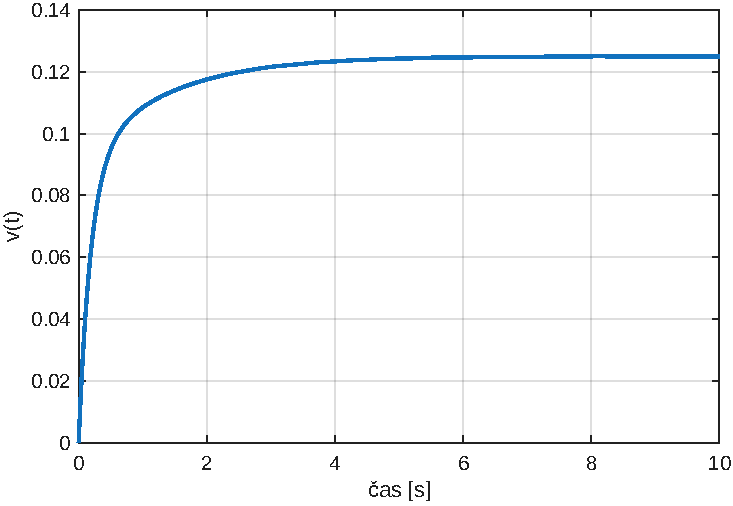
\includegraphics[width=0.8\textwidth]{img/linearizace_ii.pdf}
  \caption{Odezva linearizovaného modelu}
  \label{fig:lin1}
\end{figure}

\begin{figure}[H]
  \centering
  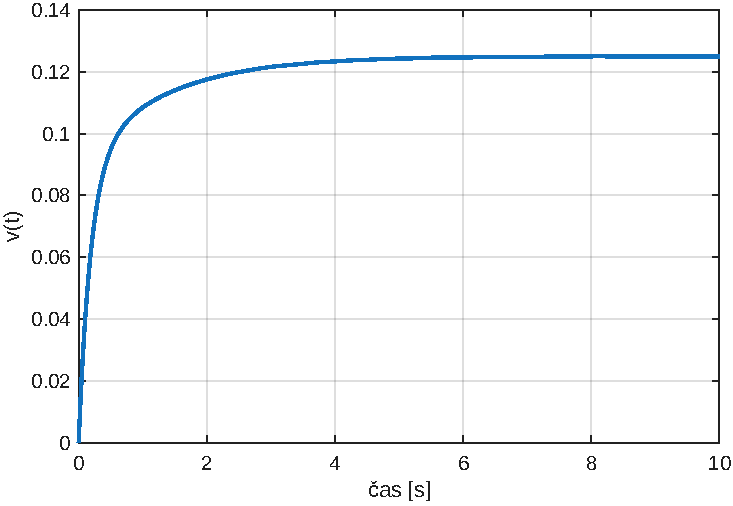
\includegraphics[width=0.8\textwidth]{img/linearizace_i.pdf}
  \caption{Odezva nelineárního modelu}
  \label{fig:nelin1}
\end{figure}

\section{Lineární aproximace modelu v prac. bodě, kde $v=10\ m/s$}
\subsection{Analytická podmínka rovnovážného pracovního bodu}

$P=(v, \omega, F)$ jsme vypočítali pomocí Matlabu obdobně jako v předchozí úloze a pro $v=10\ m/s$ jsme získali dvě řešení: $P_1=(10, 10, 400) a P_2=(1é, 1é, -400)$.

\subsection{Linearizace systému v zadaném prac. bodě}
Se statickou nelinearitou: 
\begin{lstlisting}
clear; clc;
syms v w F real

% s abs(F)
f1 = -5*v + w + 0.1*abs(F);
f2 = v - w;
f  = [f1; f2];

A_sym = jacobian(f, [v w]);
B_sym = jacobian(f, F);

v0 = 10;
w0 = 10;
F0 = 400;    % z 4a

A_i_10  = double(subs(A_sym, {v,w,F}, {v0,w0,F0}));
B_i_10  = double(subs(B_sym, {v,w,F}, {v0,w0,F0}));
C_i_10  = [1 0];
D_i_10  = 0;
\end{lstlisting}

Matice vyšly:
$$
A=\begin{bmatrix}-5 & 1 \\ 1 & -1\end{bmatrix}
\quad
B=\begin{bmatrix}0.1 \\ 0\end{bmatrix}
\quad
C=\begin{bmatrix}1 & 0\end{bmatrix}
\quad
D=0
$$

Bez statické nelinearity:
\begin{lstlisting}
clear; clc;
syms v w F real

% bez abs(F)
f1 = -5*v + w + 0.1*F;
f2 = v - w;
f  = [f1; f2];

A_sym = jacobian(f, [v w]);
B_sym = jacobian(f, F);

v0 = 10;
w0 = 10;
F0 = 400;

A_ii_10 = double(subs(A_sym, {v,w,F}, {v0,w0,F0}));
B_ii_10 = double(subs(B_sym, {v,w,F}, {v0,w0,F0}));
C_ii_10 = [1 0];
D_ii_10 = 0;
\end{lstlisting}
Zde matice vyšly:
$$
A=\begin{bmatrix}-5 & 1 \\ 1 & -1\end{bmatrix}
\quad
B=\begin{bmatrix}0.1 \\ 0\end{bmatrix}
\quad
C=\begin{bmatrix}1 & 0\end{bmatrix}
\quad
D=0
$$

\subsection{Porovnání linearizovaného modelu s původním}
Grafy \ref{fig_lin2} a \ref{fig:nelin2} jsou stejně vytvořené odezvy, jako v předchozí části:
\begin{figure}[H]
  \centering
  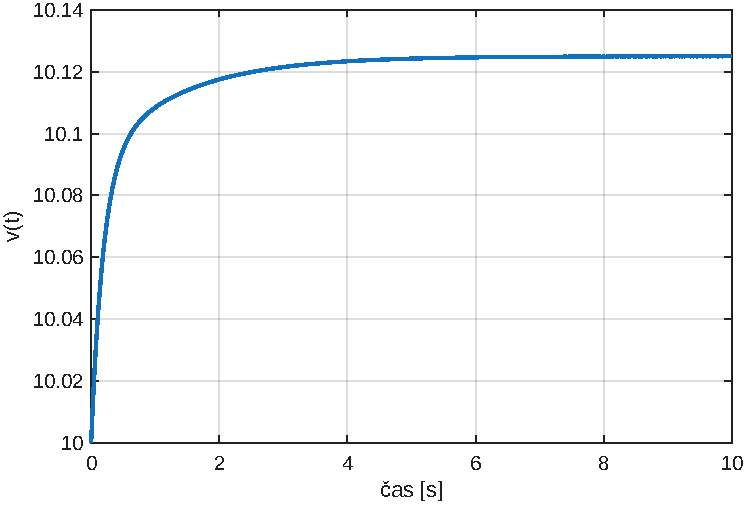
\includegraphics[width=0.8\textwidth]{img/linearizace2_ii.pdf}
  \caption{Odezva linearizovaného modelu}
  \label{fig:lin2}
\end{figure}

\begin{figure}[H]
  \centering
  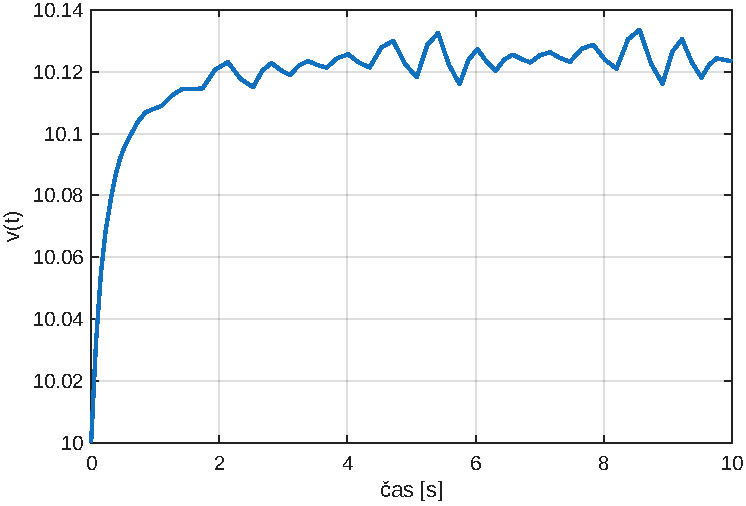
\includegraphics[width=0.8\textwidth]{img/linearizace2_i.pdf}
  \caption{Odezva nelineárního modelu}
  \label{fig:nelin2}
\end{figure}

\end{document}
